\documentclass[12pt, oneside]{article}
\usepackage[margin=0.85in]{geometry}
\linespread{1}
    
\usepackage[utf8]{inputenc}     % UTF8 encoding
\usepackage[spanish]{babel}     % Spanish words in images, tables, etc
\usepackage[dvipsnames]{xcolor} % To use colors
\usepackage{graphicx}           % For adding images
\usepackage{amsmath}            % Math extensions
\usepackage{fancyhdr}           % Header and footer

\setlength{\headheight}{14.5pt}        % Headheight changed for fancyhdr to work properly
\renewcommand{\headrulewidth}{0.4pt} % Header and footer line thickness
\pagestyle{fancy}
\fancyhead{} % Uncomment to add text to a blank header (same with fancyfoot)
\fancyhead[L]{Documentación NanoChat - Prácticas de Redes de Comunicaciones} %%% Change according to theme

%%%% Specific packages and commands for this document %%%%
\usepackage{listings}           % For displaying programming code

\renewcommand{\lstlistingname}{Código}
\definecolor{codebackground}{rgb}{0.95, 0.95, 0.95}
\definecolor{codekeywords}{rgb}{0.3,0.3,1}
%\definecolor{comments}{gray}{0.95}
\lstset{
    %language=java,                          % the language of the code
    %morekeywords={Operation,User,Users,Room,Last,Message,:,&},                  % if you want to add more keywords to the set
    %deletekeywords={...},                    % if you want to delete keywords from the given language
    %captionpos=t,                             % sets the caption-position to bottom
    %title=\lstname,                          % show the filename of files included with \lstinputlisting; also try caption instead of title
    frame=L,                            % adds a frame around the code
    %rulecolor=\color{black},                  % if not set, the frame-color may be changed on line-breaks within not-black text (e.g. comments)
    %backgroundcolor=\color{codebackground}, % choose the background color
    basicstyle=\footnotesize\ttfamily,        % the size of the fonts that are used for the code
    keywordstyle=\color{codekeywords},                % keyword style
    %commentstyle=\color{comments},            % comment style
    %stringstyle=\color{strings},              % string literal style
    %numberstyle=\tiny\color{numbers},       % the style that is used for the line-numbers
    %numbers=left,                             % possible values are (none, left, right)
    %numbersep=8pt,                            % how far the line-numbers are from the code
    %stepnumber=1,                             % the step between two line-numbers. If it's 1, each line will be numbered
    breaklines=true,                          % sets automatic line breaking
    breakatwhitespace=true,                   % sets if automatic breaks should only happen at whitespace
    %escapeinside={\%*}{*)},                  % if you want to add LaTeX within your code
    keepspaces=true,                          % keeps spaces in text, useful for keeping indentation of code (possibly needs columns=flexible)
    showspaces=false,                         % show spaces everywhere adding particular underscores; it overrides 'showstringspaces'
    showlines=true,
    showstringspaces=true,                   % underline spaces within strings only
    tabsize=4,                                % sets default tabsize to 2 spaces
    showtabs=false,                           % show tabs within strings adding particular underscores
    extendedchars=true,                       % lets you use non-ASCII characters; for 8-bits encodings only, does not work with UTF-8
    literate=
    {á}{{\'a}}1 {é}{{\'e}}1 {í}{{\'i}}1 {ó}{{\'o}}1 {ú}{{\'u}}1
    {Á}{{\'A}}1 {É}{{\'E}}1 {Í}{{\'I}}1 {Ó}{{\'O}}1 {Ú}{{\'U}}1
    {à}{{\`a}}1 {è}{{\`e}}1 {ì}{{\`i}}1 {ò}{{\`o}}1 {ù}{{\`u}}1
    {À}{{\`A}}1 {È}{{\'E}}1 {Ì}{{\`I}}1 {Ò}{{\`O}}1 {Ù}{{\`U}}1
    {ä}{{\"a}}1 {ë}{{\"e}}1 {ï}{{\"i}}1 {ö}{{\"o}}1 {ü}{{\"u}}1
    {Ä}{{\"A}}1 {Ë}{{\"E}}1 {Ï}{{\"I}}1 {Ö}{{\"O}}1 {Ü}{{\"U}}1
    {â}{{\^a}}1 {ê}{{\^e}}1 {î}{{\^i}}1 {ô}{{\^o}}1 {û}{{\^u}}1
    {Â}{{\^A}}1 {Ê}{{\^E}}1 {Î}{{\^I}}1 {Ô}{{\^O}}1 {Û}{{\^U}}1
    {œ}{{\oe}}1 {Œ}{{\OE}}1 {æ}{{\ae}}1 {Æ}{{\AE}}1 {ß}{{\ss}}1
    {ű}{{\H{u}}}1 {Ű}{{\H{U}}}1 {ő}{{\H{o}}}1 {Ő}{{\H{O}}}1
    {ç}{{\c c}}1 {Ç}{{\c C}}1 {ø}{{\o}}1 {å}{{\r a}}1 {Å}{{\r A}}1
    {€}{{\euro}}1 {£}{{\pounds}}1 {«}{{\guillemotleft}}1
    {»}{{\guillemotright}}1 {ñ}{{\~n}}1 {Ñ}{{\~N}}1 {¿}{{?`}}1
}

\definecolor{javakeywords}{rgb}{0.3,0.3,1}
\definecolor{javacomments}{rgb}{0.7,0.3,0.2}
\definecolor{javastrings}{rgb}{0.7,0.2,0.7}
\lstdefinestyle{JavaStyle}{
    language=java,                          % the language of the code
    frame=L,                            % adds a frame around the code
    rulecolor=\color{black},                  % if not set, the frame-color may be changed on line-breaks within not-black text (e.g. comments)
    %backgroundcolor=\color{codebackground}, % choose the background color
    basicstyle=\footnotesize\ttfamily,        % the size of the fonts that are used for the code
    keywordstyle=\color{javakeywords},                % keyword style
    commentstyle=\color{javacomments},            % comment style
    stringstyle=\color{javastrings},              % string literal style
    %numberstyle=\tiny\color{numbers},       % the style that is used for the line-numbers
    %numbers=left,                             % possible values are (none, left, right)
    %numbersep=8pt,                            % how far the line-numbers are from the code
    %stepnumber=10,                             % the step between two line-numbers. If it's 1, each line will be numbered
    tabsize=4,                                % sets default tabsize to 2 spaces
    showstringspaces=false,                   % underline spaces within strings only
    captionpos=t,                             % sets the caption-position to bottom
    %title=\lstname,                          % show the filename of files included with \lstinputlisting;
    columns=flexible,
}

\usepackage{multicol} 
\usepackage{array}
\usepackage{multirow}
\usepackage{hyperref}
\usepackage{verbatim}
\usepackage{upquote}
\usepackage{float}
\usepackage{scrextend}
\usepackage{enumitem}
\newcommand{\keyw}[1]{\textbf{#1}}
\newcommand{\mess}[1]{\hyperref[message:#1]{#1}}
%\newcommand{\comm}[1]{\textbf{#1}}
\newcommand{\comm}[1]{{\textcolor{MidnightBlue}{\fontsize{13pt}{13pt} \texttt{#1}}}}



\begin{document}
\begin{titlepage}
    \begin{center}
        \vspace*{1cm}
        
        \Huge
          \textbf{NanoChat}
        
        \vspace{0.5cm}
        \LARGE
        \textbf{Diseño de un servidor de chat}
        
        \vspace{1.5cm}
        
   		  \vspace{1.5cm}
        
        \textbf{Redes de comunicaciones}\\
        \textbf{Convocatoria Junio 2018/2019}
       
        \vfill
        
        %Obor XY
        
        \vspace{0.8cm}
          \Large
          \begin{flushright}
          	\begin{tabular}{lr}
              Autores:&Emilio Domínguez Sánchez \\ &José Manuel Ruiz Ródenas \\
              Profesor:&Oscar Cánovas Reverte\\
              Grupo:& PCEO \\
              %Usuario Mooshak: & D32 \\
              %Convocatoria:&Junio 2018 \\
            \end{tabular}
          \end{flushright}
        \vspace{0.5cm}
       Abril de 2019
        
    \end{center}
\end{titlepage} % title file
\addtocontents{toc}{~\hfill\textbf{Page}\par}
\tableofcontents
\newpage
\section{Introducción}
Esta es la memoria del proyecto de prácticas de la asignatura de Redes de Comunicaciones. El proyecto se basa en el diseño e implementación de un sistema de mensajería, de nombre \keyw{NanoChat}, que consta de: un directorio, servidores que responden a ciertos protocolos predefinidos y un grupo de clientes que se conectan a ellos; aunque de aquí en adelante cuando hablemos de la aplicación NanoChat nos referiremos a la aplicación cliente. \\

La especificación de la pŕactica se encuentra adjunta junto con esta memoria en el archivo que se incluye. El funcionamiento resumido es el siguiente: la aplicación de usuario se comunica con el directorio y pide un servidor de chat que utilice un protocolo de comunicación específico; a lo que el directorio responde con los datos necesarios para conectarse a un servidor de chat y con ellos se inicia la comunicación con ese servidor. Es decir, los servidores de chat deben registrar su dirección de red  y el protocolo que utilizan en el directorio. Además, puede haber varios servidores de chat que utilicen el mismo protocolo, por tanto, cada vez que un usuario pida la dirección de red de un servidor de un protocolo en específico, se le devolverá la dirección de un servidor cualquiera que cumpla los requisitos. \\

Nuestro trabajo ha consistido en diseñar el protocolo de comunicación del directorio y un protocolo de chat para un servidor concreto, y programar aplicaciones que los implementen.

\subsection{Funcionalidad. Manual de usuario de la aplicación NanoChat.}
En esta sección vamos a explicar cómo funciona nuestra aplicación de chat y qué funcionalidades proporciona.

\subsubsection{Inicio y registro}
Una vez ejecutada la aplicación de \keyw{NanoChat}, se permite el acceso a una línea de comandos con la cual interactuaremos con el servidor de chat. El listado completo de las órdenes lo podemos encontrar en una lista proporcionada por el comando \comm{help}, que se puede ejecutar en cualquier momento. El primer paso será registrarse en el servidor de chat. Para ello, ejecutaremos el comando \comm{nick <nick elegido>}. Puede ser que el nick que hemos elegido ya esté siendo usado, si ese es el caso debemos volver a intentarlo con un nick distinto.

\subsubsection{Fuera de una sala}
Una vez registrados en el servidor podemos hacer uso de los siguientes comandos de aplicación:
\begin{itemize}[align=left]
    \item [\comm{roomlist}:] Imprime por pantalla la lista de salas registradas en el servidor mostrando: su nombre, usuarios que se encuentran  dentro y el momento del último mensaje enviado.
    \item [\comm{enter <nombre de la sala>}:] Permite acceder a una sala de chat.
    \item [\comm{create <nombre de la sala>}:] Permite registrar una sala de chat en el servidor y una vez registrada se accede a ella automáticamente con el rol de administrador.
    \item [\comm{dm <usuario> {} <mensaje>}:] Envía un mensaje privado a un usuario registrado en el servidor (también se puede usar dentro de las salas de chat). 
\end{itemize}

\subsubsection{Dentro de una sala}
Las salas de chat son lugares donde los usuarios pueden mandarse mensajes de manera grupal. En este servidor de chat hemos implementado dos tipos distintos de salas:

\begin{itemize}
    \item \textit{Salas temporales:} son creadas por los usuarios con el comando \comm{create}. Si estas salas se quedan sin usuarios son borradas del servidor. En ellas, existe el rol de administrador, que en un principio se otorga al creador de la sala. El rol de administrador permite el uso de los siguientes comandos:
    
    \begin{itemize}[align=left]
        \item [\comm{promote <usuario>:}] Concede al usuario seleccionado el rol de administrador (el usuario candidato debe estar en la misma sala), el rol de administrador se pierde si el usuario sale de la sala.
        \item [\comm{kick <usuario>:}] Expulsa de la sala al usuario seleccionado.
        \item [\comm{rename <nuevo nombre>:}] Permite cambiar el nombre de la sala. En el caso de que exista otra sala con el nombre elegido, este no se cambiará.
    \end{itemize}
    
    \item \textit{Salas globales:} son las salas predefinidas por el servidor, no tienen rol de administrador, por lo que estas salas tendrán siempre el mismo nombre y en ellas no se podrá expulsar a nadie. En concreto, este servidor de chat tiene dos salas de este tipo por defecto: \keyw{General} y \keyw{PublicBar}.
    
\end{itemize}
Dentro de cualquier tipo de sala, podemos usar los siguientes comandos:
\begin{itemize}[align=left]
    \item [\comm{info}:] Imprime por pantalla la información de la sala con el mismo formato que \comm{roomlist}.
    \item [\comm{send <mensaje>}:] Permite enviar un mensaje a la sala. %TODO ver si poner que no dejará enviar un mensaje con ciertos caracteres (dependerá de la implementación)
    \item [\comm{dm <usuario> {} <mensaje>}:] Envía un mensaje privado a otro usuario registrado en el servidor.
    \item [\comm{exit}:] Permite al usuario salir de la sala en la que se encuentra.
\end{itemize}

\subsubsection{Salir y cerrar la aplicación}
El comando \comm{quit} se puede ejecutar en cualquier momento y desconecta al usuario del servidor, quedando su nick disponible para otro usuario que entre al servidor.

\section{Diseño de los protocolos de comunicación}
La parte central del proyecto se basa en diseñar (e implementar) un protocolo de comunicación entre un cliente de chat y el servidor, pasando por el paso previo de comunicarse con el directorio, el cual hemos diseñado pensando en la funcionalidad descrita anteriormente.

Para describir los protocolos, nos basaremos en autómatas. Cada nodo de un autómata representa el estado de una comunicación en un momento concreto, y las flechas que salen de ese nodo representan qué tipo de eventos se pueden dar en ese estado y por qué se dan. Las eventos pueden producirse por el envío o la recepción de mensajes y el final de la flecha representa el nuevo estado de la comunicación a continuación. Por ejemplo, hay puntos en la comunicación donde el cliente puede enviar un mensaje solicitando una lista de las salas disponibles en el servidor, y pasa entonces a un estado de espera de la respuesta. El envío y la recepción de mensajes se representan en la arista con las letras \lstinline!send! y \lstinline!rcv! respectivamente.

\subsection{Protocolo de comunicación con el directorio}
La comunicación con el directorio utiliza como protocolo de red UDP, tal como se indicó en las clases. Si bien el canal es no confiable, para la facilitación del proyecto se ha supuesto que este ofrece ciertas garantías (no entrega paquetes retrasados o duplicados).

El protocolo que hemos diseñado es bastante simple: un servidor de chat que quiera registrarse en el directorio manda una mensaje de tipo \lstinline!REGISTER! con sus datos, y si el directorio recibe el datagrama de forma correcta, el servidor será registrado y se le contestará con mensaje de tipo \lstinline!ACK!. Los clientes de chat por su parte envían una solicitud de tipo \lstinline!QUERY!, a la que el servidor responde con una solicitud de tipo \lstinline!INFO! o \lstinline!NOT_FOUND!.

\subsubsection{Autómata del servidor de directorio}
El autómata siguiente representa el funcionamiento del directorio. Es el autómata más simple de los tres, pues solo espera consultas y responde apropiadamente. En la imagen se pueden observar sus 3 estados: el estado de reposo, representado como \lstinline{INIT}, donde empieza su actividad (suponemos que acaba con la desconexión del servidor); y dos estados más, correspondientes a cuando se reciben solicitudes de un servidor de chat para registrarse en el directorio (\lstinline{REGISTER}) y cuando se reciben solicitudes de un cliente de chat pidiendo la dirección de algún servidor registrado (\lstinline{QUERY}).

\begin{center}
    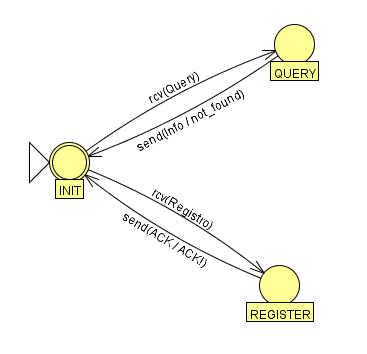
\includegraphics[width=200pt]{Images/Automata_Directorio.png}    
\end{center}

\subsubsection{Formato de los mensajes} %TODO Conciso y sencillo
A continuación mostramos el formato de los distintos mensajes de directorio. Siguiendo las condiciones exigidas en esta entrega de prácticas, hemos utilizado codificación en binario, mientras que los mensajes del \keyw{servidor de chat}, que veremos más adelante, se han diseñado en formato de texto plano. Todos los mensajes contienen una cabecera de 1 byte con el código de operación (OpCode), y una serie de campos de longitud fija.

\begin{table}[H]
\begin{tabular}{l l}
    \textit{Mensaje \lstinline!REGISTER!} &
        \begin{tabular}{|c|c|c|c|}\hline
             OpCode & Puerto servidor & ID del protocolo \\ \hline
             0x10 & 4 bytes & 1 byte \\ \hline %hexadecimal
        \end{tabular}
    \\
\end{tabular}
\end{table}

Es importante notar que no es necesario codificar en el mensaje \lstinline!REGISTER! la dirección IP del servidor, pues la podemos obtener a través de la cabecera de la capa de red del paquete recibido.

\begin{table}[H]
\begin{tabular}{l l}
    \textit{Mensaje \lstinline!QUERY!} &
        \begin{tabular}{|c|m{3cm}|}\hline
             OpCode & ID del protocolo \\ \hline
             0x8 & 1 byte \\ \hline
        \end{tabular}
    \\
    \textit{Mensaje \lstinline!INFO!} &
        \begin{tabular}{|c|m{3cm}|l|}\hline
             OpCode & IP del servidor &  Puerto \\ \hline
             0x4 & 4 bytes (IPv4) & 4 bytes \\ \hline
        \end{tabular}
    \\
    \textit{Mensaje \lstinline!NOT_FOUND!} &
        \begin{tabular}{|c|}\hline
             OpCode  \\ \hline
              0x2 \\ \hline
        \end{tabular}
    \\
    \textit{Mensaje \lstinline!ACK!} &
        \begin{tabular}{|c|}\hline
             OpCode \\ \hline
             0x0 \\ \hline
        \end{tabular}
    \\
\end{tabular}
\end{table}

\subsubsection{Ejemplos de comunicación}
Vamos a ver un ejemplo de comunicación para un directorio en funcionamiento, para mostrar el uso correcto de los mensajes anteriores. Para empezar, supongamos que un servidor de chat tiene disponible un servicio con un protocolo que se identifica con el código $87$ en el puerto $196$ y quiere registrarse. Entonces enviaría el siguiente mensaje de tipo \lstinline!REGISTER!:
\begin{center}
\begin{tabular}{|c|c|c|c|}\hline
    OpCode & Puerto servidor & ID del Protocolo \\ \hline
    0x10 & 196 & 87 \\ \hline %hexadecimal
\end{tabular}
\end{center}
El servidor debería establecer algún tiempo de timeout por si el paquete se perdiese reenviarlo. Cuando el directorio reciba el paquete, enviará un mensaje \lstinline!ACK!. Si el paquete de respuesta se perdiese, saltaría el tiempo de timeout, y el servidor debe intentar registrarse de nuevo. Una vez recibido el \lstinline!ACK!, el servidor sabe que ha sido registrado.

Continuando con el ejemplo, imaginemos que más tarde un cliente quiere conectarse a un servidor de chat de código $87$, y envía el siguiente mensaje al servidor de tipo \lstinline!QUERY!:
\begin{center}
\begin{tabular}{|c|c|}\hline
    OpCode & ID del Protocolo \\ \hline
    0x8 & 87 \\ \hline
\end{tabular}
\end{center}
Al igual de antes, el cliente debe considerar un tiempo de timeout después del cuál supone que el paquete no ha llegado. Al llegar, el directorio reconoce que tiene un servidor registrado que implementa el protocolo de chat. Por tanto, responde con un comando \lstinline!info! con la IP y el puerto del servidor, que sacó del mensaje que recibió previamente. Suponiendo que el servidor tuviese por IP 107.94.28.2, el cliente recibiría este mensaje:
\begin{center}
\begin{tabular}{|c|c|c|}\hline
    OpCode & IP servidor  &  Puerto servidor \\ \hline
    0x4 & 107.94.28.2 & 196 \\ \hline
\end{tabular}
\end{center}
Con esta información, el cliente puede comunicarse con el servidor de chat.

\subsection{Protocolo del servidor de chat}
El protocolo inventado para un supuesto servidor de chat consiste en la parte fundamental del proyecto y lo hemos diseñado pensando en la funcionalidad que queríamos ofrecer al usuario.

\subsubsection{Autómata del cliente de chat}
La figura \ref{aut_cliente} muestra el autómata que representa al proceso cliente, el cual da acceso al usuario al servidor de chat. Los dos primeros estados corresponden con la conexión que se establece entre cliente y directorio y posteriormente el registro del usuario en el servidor de chat.

\begin{figure}[H]
    \makebox[\textwidth]{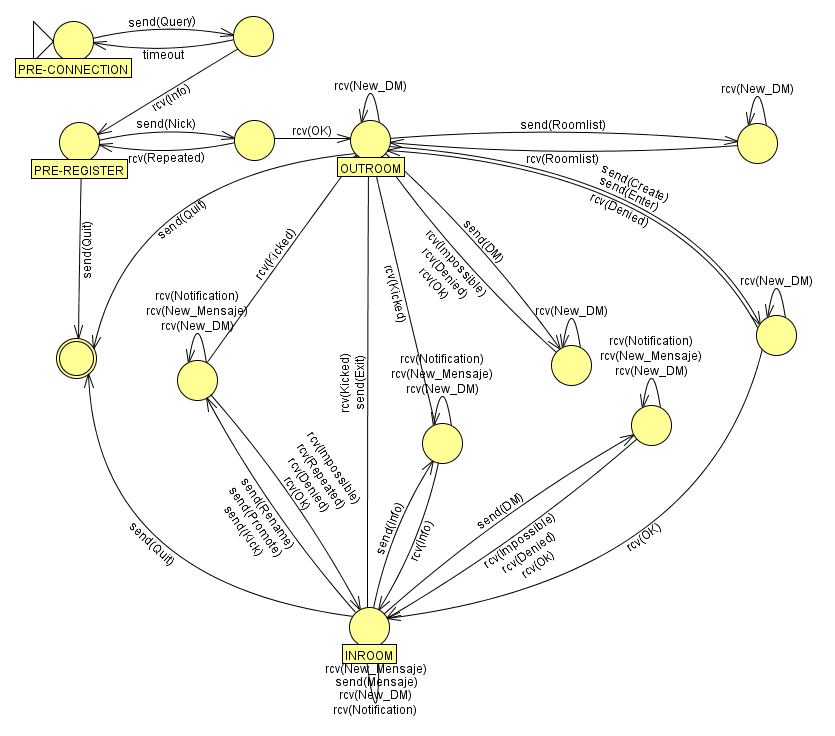
\includegraphics[width=1.1\textwidth]{Images/AutomataClienteFinalisimo.png}}
    \caption{Autómata del cliente de chat.}
    \label{aut_cliente}
\end{figure}

\begin{itemize}
    \item \lstinline!PRE-CONNECTION!: Es el estado inicial del autómata. Desde él, el cliente solicita al \keyw{directorio} una dirección IP para un servidor de chat que utilice su protocolo. Una vez el cliente manda la consulta y consigue una dirección válida, pasa al estado \lstinline!PRE-REGISTER!. Hemos diseñado el cliente de forma que esta parte se ejecuta automáticamente sin intervención del usuario una vez se inicia el cliente, y nunca más se vuelve a este estado.
    \item \lstinline!PRE-REGISTER!: Una vez se llega a este estado, el cliente puede interactuar con el servidor de chat. A partir de aquí el usuario puede llevar a cabo las acciones descritas en el manual de usuario. Es decir, lo primero será registrarse con el comando \comm{nick}. A este estado no se podrá volver una vez registrado.
\end{itemize}

El resto de estados se basan en lo descrito en el manual. Por simplicidad con los términos, hemos dado a los mensajes (dentro de lo posible) el mismo nombre que la funcionalidad que representan. Tenemos dos estados principales, que son \lstinline{OUTROOM} e \lstinline{INROOM}, que se corresponden con que el cliente esté fuera o dentro de una sala. Los estados sin nombre son momentos en los que, tras una consulta al servidor (entrar a una sala, echar a alguien de una sala, etc), el cliente espera el resultado de su consulta.

Aunque hemos dicho que el autómata se entiende a raíz de la funcionalidad presentada, en la imagen se pueden ver transiciones que, en principio, no parece que correspondan con lo que se expone. Por ejemplo, se puede recibir un mensaje de otro usuario mientras se espera la respuesta al comando\comm{info}. ¿Cómo es esto posible? Esta situación se puede dar porque en cualquier momento otro usuario puede escribir en el chat. El autómata del cliente espera la respuesta a un comando, pero puede recibir mensajes de sala, notificaciones, etc. En estas situaciones, podemos programar la aplicación para que muestre por pantalla el mensaje en el momento en que llega, o que muestre primero el resultado de la consulta.


\subsubsection{Autómata del servidor de chat}
La figura \ref{aut_servidor} representa el autómata de uno de los \keyw{hilos del servidor de chat} que atiende a un cliente cualquiera. Como vemos, tiene once estados, de los cuales tres de ellos han sido marcados con un nombre. Estos nombres coinciden con los que hemos puesto en el autómata anterior con la finalidad de remarcar el paralelismo que existe entre ambos (también hemos querido reflejarlo con la representación gráfica de ambos); ya que los mensajes que se pueden atender dependen del estado del otro autómata.

\begin{figure}{H}
    \makebox[\textwidth]{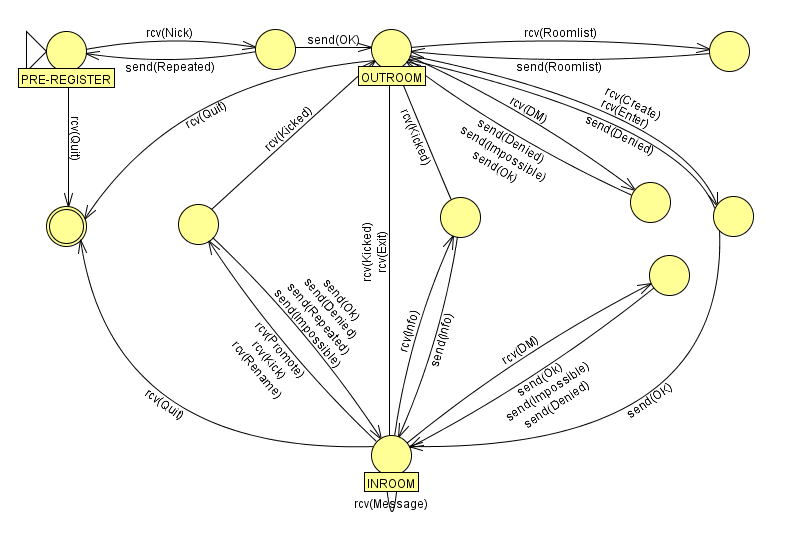
\includegraphics[width=1.1\textwidth]{Images/AutomataServidorFinalisimo.png}}
    \caption{Autómata del servidor de chat.}
    \label{aut_servidor}
\end{figure}

\subsubsection{Mensajes de chat}
Como se nos ha pedido mientras elaborábamos la práctica, los mensajes del \keyw{servidor de chat} siguen el formato \keyw{Field-Value}.

El formato de mensajes Field-Value codifica la información que va dentro de un mensaje en \keyw{campos}; determinados por un nombre, por ejemplo \lstinline!Operation!; a los que se asigna un valor; que para el campo \lstinline!Operation!, que representa el tipo de operación, podría ser \lstinline!Create!. Los mensajes contienen el nombre de cada campo y su valor en una línea, separados por un delimitador; en nuestro caso, el carácter dos puntos (\lstinline!:!). Como requisito, el mensaje debe acabar siempre con una línea vacía.

Además, se pueden diseñar mensajes en los que importe o no el orden en el que se escriben los campos y en los que un campo admita varios valores separados por un separador. En nuestro caso, en todos nuestros mensajes se debe respetar el orden que se establece en los campos, y también hemos diseñado algunos mensajes que admiten varios valores separados por el carácter ampersand (\lstinline{&}).

Como los mensajes se separan por líneas y además se usa un carácter especial para el delimitador y otro para el separador, hay que ver cómo formatear mensajes en los cuales pueden aparecer estos caracteres en los valores de los campos. En nuestro caso, no permitimos el uso del carácter final de línea en ningún sitio. Es decir, no se pueden registrar usuarios o salas que contengan un final de línea en su nombre o enviar mensajes de varias líneas. Igualmente, el delimitador tampoco puede estar presente en los nombres de los campos pero sí en los valores, de forma que el nombre del campo se interpreta desde el principio de la línea hasta el primer carácter delimitador encontrado. Y por último, los valores que estén divididos por el separador no pueden contener éste carácter. No obstante, aunque el protocolo no lo exige, en nuestra implementación no permitimos que los nombres de usuario y sala contengan caracteres en blanco (espacios, tabuladores, etc).

\subsubsection*{Ejemplos de comunicación}
Por ejemplo, el primer comando que usa un cliente al entrar al servidor es el comando \comm{nick}. Al usar este comando, el cliente manda un mensaje al servidor indicando que quiere registrarse con un \keyw{nickname} específico. Como veremos en el \hyperref[sec:listado]{listado de mensajes}, el mensaje \mess{Register} cuenta con dos campos; el campo \lstinline{Operation}, común a todos los mensajes y que codifica el tipo de operación, y el campo \lstinline!User!, que contiene el nombre de usuario. Por tanto, para registrarse con el \keyw{nickname} Alberto, se mandaría un mensaje como el siguiente (atención a la línea en blanco al final):

\begin{lstlisting}
Operation:Register
User:Alberto

\end{lstlisting}

A este mensaje el servidor podría responder con un mensaje de tipo \mess{Ok}, \mess{Denied} o \mess{Repeated}, en función de si se pudo registrar, el nombre no es válido o ya había un usuario con ese nombre. La respuesta habitual sería recibir un mensaje del siguiente tipo:

\begin{lstlisting}
Operation:Ok

\end{lstlisting}

Ilustremos ahora otro ejemplo donde el mensaje recibido por el cliente es más complejo. En el estado \lstinline{OUTROOM}, el cliente puede mandar un mensaje \mess{List Rooms} para solicitar la lista de salas del servidor.

\begin{lstlisting}
Operation:Get room list

\end{lstlisting}

El hilo del servidor que atiende a éste usuario reunirá la información necesaria para enviarle un mensaje con la descripción de cada sala. Se trata del mensaje \mess{Rooms List} (es conveniente leer el formato que sigue este mensaje). Este mensaje es más complejo porque, primero, no tiene una longitud (en líneas) fija, sino que depende del número de salas que haya. Segundo, cada sala se codifica con tres campos distintos, por lo que fuerza a que exista un orden en los campos, o no sabríamos qué salan pertenecen. Y tercero, el campo \lstinline{Users} de cada sala es un campo múltiple que puede contener varios nombres. Una respuesta a la petición anterior podría ser:

\begin{lstlisting}
Operation:Room List
Room:Sala1
Users:Alberto&Javi&shanon
Last Message:104958
Room:SalaVacia
Users:
Last Message:0
Room:SalaNuevaDeEnrique
Users:Enrique
Last Message:0
Room:SalaGlobal
Users:
Last Message:20456788

\end{lstlisting}
\subsubsection{Listado de los mensajes del servidor de chat}
A continuación mostramos el listado de todos los mensajes que componen nuestra aplicación y su uso en relación al autómata.
%%%% Comandos

\newcommand{\str}[1]{\texttt{\char`\"}\texttt{#1}\texttt{\char`\"}}

\newenvironment{displayMessage}[1]
{\renewcommand{\arraystretch}{1.3} % General space between rows (1 standard)
\begin{table}[H]
    \centering
    \refstepcounter{table}\label{message:#1}
    \begin{tabular}{|l p{0.7\textwidth}|}
    \multicolumn{2}{c}{\large Mensaje #1} \\
    \hline
}
{
    \hline
    \end{tabular}
\end{table}
}
\definecolor{opColor}{rgb}{0.9,0.6,0.1}
\newenvironment{displayControlMessage}[2]
{
\begin{displayMessage}{#1}
Formato: &  \begin{tabular}{l l}
                Operation:      & \str{#2} \\
            \end{tabular} \\
\hline
Descripción: &
}
{
 \\
\end{displayMessage}
}

%%%% Comienzo
\label{sec:listado}

\begin{displayMessage}{Register}
Formato: &  \begin{tabular}{l l}
                Operation:  & \str{Register} \\
                User:       & \str{<username>} \\
            \end{tabular} \\
\hline
Descripción: & Mensaje para registrar un \keyw{nickname} en el servidor de chat. \\

Uso:         & El mensaje solo puede ser enviado cuando el cliente se encuentra en el estado \lstinline!PRE-REGISTER!.  El nickname no puede contener el carácter separador (\lstinline!&!).\\
\end{displayMessage}
\begin{displayControlMessage}{List Rooms}{Get room list}
Mensaje de control que envía el cliente cuando solicita la lista de salas.
\end{displayControlMessage}
\begin{displayMessage}{Create}
Formato: &  \begin{tabular}{l l}
                Operation:      & \str{Create} \\
                Room:           & \str{<room name>} \\
            \end{tabular}\\
\hline
Descripción: & Mensaje para crear una \keyw{sala} en el servidor de chat. \\
\end{displayMessage}
\begin{displayMessage}{Rename}
Formato: &  \begin{tabular}{l l}
                Operation:      & \str{Rename} \\
                New name:       & \str{<room name>} \\
            \end{tabular}\\
\hline
Descripción: & Mensaje para renombrar una \keyw{sala} en el servidor de chat. \\
\end{displayMessage}
\begin{displayMessage}{Enter}
Formato: &  \begin{tabular}{l l}
                Operation:      & \str{Enter} \\
                Room:           & \str{<room name>} \\
            \end{tabular}\\
\hline 
Descripción: & Mensaje para entrar en una \keyw{sala} del servidor de chat. \\
\end{displayMessage}
\begin{displayControlMessage}{Info}{Get info}
Mensaje de control que envía el cliente cuando solicita la información detallada de la sala en la que se encuentra.
\end{displayControlMessage}
\begin{displayMessage}{Promote}
Formato: &  \begin{tabular}{l l}
                Operation:      & \str{Promote} \\
                User:           & \str{<username>} \\
            \end{tabular}\\
\hline
Descripción: & Mensaje para hacer \keyw{administrador de sala} a otro usuario. \\
\end{displayMessage}
\begin{displayMessage}{Kick}
Formato: &  \begin{tabular}{l l}
                Operation:      & \str{RICKROLL} \\
                User:           & \str{<username>} \\
            \end{tabular}\\
\hline
Descripción: & Mensaje para echar de una sala a otro usuario. \\
\end{displayMessage}
\begin{displayMessage}{Send}
Formato: &  \begin{tabular}{l l}
                Operation:      & \str{Send} \\
                Text:           & \str{<message>} \\
            \end{tabular}\\
\hline
Descripción: & Mensaje que envía el cliente para enviar un mensaje de chat cuando está en una sala. \\
\end{displayMessage}
\begin{displayMessage}{DM}
Formato: &  \begin{tabular}{l l}
                Operation:      & \str{DM} \\
                User:           & \str{<username>} \\
                Text:           & \str{<message>} \\
            \end{tabular}\\
\hline
Descripción: & Mensaje directo del cliente hacia otro usuario en específico. \\
\end{displayMessage}
\begin{displayControlMessage}{Exit}{Exit room}
Mensaje de control que envía el cliente para salir de una sala.
\end{displayControlMessage}
\begin{displayControlMessage}{Quit}{Quit}
Mensaje de control que envía el cliente al dejar el servidor.
\end{displayControlMessage}




\begin{displayControlMessage}{Ok}{Ok}
Mensaje de control que indica que una operación se llevó a cabo correctamente.
\end{displayControlMessage}
\begin{displayControlMessage}{Denied}{Denied}
Mensaje de control que indica que una operación no se pudo realizar porque no le está permitida al usuario. Por ejemplo, podría ser una respuesta del servidor al renombrar una sala en la que no tiene permisos o introducir un \keyw{nickname} que contiene algún caracter ilegal.
\end{displayControlMessage}
\begin{displayControlMessage}{Repeated}{Repeated}
Mensaje de control que indica que una operación no se pudo realizar porque no preserva la unicidad de algún elemento. Por ejemplo, podría ser una respuesta del servidor al intentar renombrar una sala con un nombre de otra sala ya existente.
\end{displayControlMessage}
\begin{displayControlMessage}{Impossible}{Impossible}
Mensaje de control que indica que una operación no se pudo realizar porque no es posible. Por ejemplo, podría ser una respuesta del servidor al intentar echar a un usuario de una sala cuando el usuario no está en la sala.
\end{displayControlMessage}
\begin{displayControlMessage}{Kicked}{YOU GOT RICKROLLED}
Mensaje de control que le llega a un usuario cuando ha sido expulsado de una sala.
\end{displayControlMessage}
\begin{displayMessage}{Rooms List}
Formato: &  \begin{tabular}{l l}
                Operation:      & \str{Rooms List} \\
                Room:           & \str{<room name>} \\
                Users:          & \str{<username>\&<username>\&\ldots\&<username>} \\
                Last Message:   & \str{<last message time>} \\
                \multicolumn{2}{c}{\ldots} \\
                Room:           & \str{<room name>} \\
                Users:          & \str{<username>\&<username>\&\ldots\&<username>} \\
                Last Message:   & \str{<last message time>} \\
            \end{tabular}\\
\hline
Descripción: & Este mensaje lista las salas del servidor junto con su información básica. Para cada sala en el servidor, vienen tres campos consecutivos. El campo \lstinline!Room! contiene el nombre de la sala, el campo \lstinline!Users! contiene los usuarios que hay dentro de la sala o nada si no hay ninguno y el campo \lstinline!Last Message! contiene la fecha del último mensaje codificada en milisegundos transcurridos desde 1970. Para codificar que nadie ha escrito aún en la sala, el campo \lstinline!Last Message! debe valer 0. \\
\end{displayMessage}
\begin{displayMessage}{Rooms Info} %TODO completar
Formato: &  \begin{tabular}{l l}
                Operation:      & \str{Room info} \\
                Room:           & \str{<room name>} \\
                Users:          & \str{<username>\&<username>\&\ldots\&<username>} \\
                Last Message:   & \str{<last message time>} \\
            \end{tabular}\\
\hline
Descripción: & Este mensaje lista la información detallada de la sala en la que nos encontramos. Los campos \lstinline!Room!, \lstinline!Users! y \lstinline!Last Message! siguen el formato del mensaje \mess{Rooms List}. \\
\end{displayMessage}
\begin{displayMessage}{New Message}
Formato: &  \begin{tabular}{l l}
                Operation:      & \str{New text message} \\
                User:           & \str{<username>} \\
                Text:           & \str{<text>} \\
            \end{tabular}\\
\hline
Descripción: & Mensaje enviado por el servidor a un cliente cuando otro usuario de su sala escribió en el chat.\\
\end{displayMessage}
\begin{displayMessage}{New DM}
Formato: &  \begin{tabular}{l l}
                Operation:      & \str{New DM} \\
                User:           & \str{<username>} \\
                Text:           & \str{<text>} \\
            \end{tabular}\\
\hline
Descripción: & Mensaje enviado por el servidor a un cliente cuando otro usuario le escribe un mensaje secreto.\\
\end{displayMessage}
\begin{displayMessage}{Notification}
Formato: &  \begin{tabular}{l l}
                Operation:      & \str{Action} \\
                User:           & \str{<username>} \\
                Action:         & \str{<operation>} \\
                Object:         & \str{<object>} \\
            \end{tabular}\\
\hline
Descripción: & Mensaje enviado por el servidor a un cliente para notificarle de un evento que sucede en su sala, como que un usuario echó a otro de la sala. \\
Uso: & Ejemplo de un mensaje que notifica de la expulsión del usuario \str{alb} de la sala por parte de \str{fern}: 
\begin{lstlisting}
Operation:Action
User:fern
Action:Kicked
Object:alb

\end{lstlisting} \\
\end{displayMessage}






\section{Detalles principales de la implementación} 
Finalmente entraremos en detalle sobre la implementación de la práctica. Para la evaluación, se nos exigía una funcionalidad básica y la implementación de algunas mejoras podían mejorar nuestra calificación. Las mejoras corresponden a la implementación de mensajes directos, administradores en las salas, notificaciones de sala y la creación de nuevas salas. También se tratan de mejoras pequeñas la implementación de varios tipos de sala y definir más mensajes de control para el servidor, para notificar distintos tipos de situaciones. Por ejemplo, recibiremos un mensaje de tipo \mess{Repeated} si intentamos hacer administrador a un usuario que ya lo es.

Otra cosa que queremos comentar es que hemos cambiado gran parte del código inicial del proyecto. Aunque la estructura del proyecto es esencialmente la misma, con las mismas clases, hemos modificado muchas opciones para dejarlas como creemos que es adecuado. Por ejemplo, hemos añadido enumerados en sitios donde se usaban códigos como constantes o hemos cambiado la implementación de los mensajes para que sea más difícil cometer fallos programando y se detecten fallos en la codificación.

Las ideas para la implementación de la funcionalidad básica se pueden encontrar en la especificación de la misma. A continuación, comentaremos la implementación de los cambios más importantes.

\subsection{Representación de los mensajes} %TODO hablar de como se ha transformado la clase NCMessage entodo lo que es ahora y explicar decisión de hacer clases distintas, encoder, decoder, excepciones
Cuando empezamos con el proyecto y a diseñar el protocolo de comunicación, nos dimos cuenta de que muchos mensajes iban a compartir formato. Por ejemplo, los mensajes \mess{Register}, \mess{Create}, \mess{Enter}, y otros tantos envían solo una cadena de texto (además del tipo de operación). Es más, en esos $3$ mensajes, el nombre de ese campo podría haber sido <<name>>, pues la cadena se corresponde con el nombre de un usuario o de una sala. De hacerlo así, en la aplicación podríamos haber tenido una única clase para representar todos estos mensajes.

Los motivos por los que no lo hemos ni diseñado ni implementado así son varios. El primero, es que pensamos que, en este caso, no se debe diseñar el protocolo pensando en que sea fácil de implementar. En su lugar, debería ser fácil entender los mensajes. No hay ningún motivo, desde el punto de vista de la comunicación, para no llamar al campo del mensaje \mess{Create} <<room>>. Entre estas dos opciones:

\begin{multicols}{2}
\begin{lstlisting}
Operation:Create
Room:A

\end{lstlisting}
     \columnbreak
\begin{lstlisting}
Operation:Create
Name:A

\end{lstlisting}
\end{multicols}

en en el primer caso queda claro que se crea una sala con nombre <<A>>, mientras que en el segundo caso no sabemos qué se crea, solo que se llama <<A>>.

Por otro lado, si una misma clase representa varios tipos de mensajes en la aplicación, es sencillo que al programar, cuando representaba un tipo de mensaje, se use como otro. En cambio, si una clase se llama \lstinline!NCDirectMessage!, es evidente qué tipo de mensaje representa. Por tanto, hemos diseñado los mensajes del protocolo buscando la semántica para los campos que más facilitase la lectura, y hemos implementado, para cada tipo de mensaje, una clase distinta.

Con todo y eso, cuando se va a implementar una clase distinta para cada mensaje, no se quiere tener que repetir mucho código, porque de cambiarlo en un sitio, hay que modificarlo en todos, lo cual, además de consumir tiempo, fomenta cometer un error. Por tanto, cogimos la parte fundamental de las clases de los mensajes, que son las funciones que codifican y decodifican un mensaje, e hicimos dos clases externas que realizasen esta tarea. Estas clases se llaman \lstinline!NCMessageEncoder! y \lstinline!NCMessageDecoder!. De esta manera, la implementación de nuevos mensajes es también muy simple. Por ejemplo, el código del mensaje \mess{Create} es así de simple:

\lstinputlisting[style=JavaStyle, caption=NCCreateMessage]{../../src/messageFV/messages/NCCreateMessage.java}

\subsubsection*{La clase NCMessageEncoder}
La clase \lstinline{NCMessageEncoder} abstrae la codificación de un mensaje \keyw{Field-Value} cualquiera. Posee métodos para codificar campos simples y múltiples, y sigue un patrón de diseño común en la programación orientada a objetos llamado \keyw{builder pattern} en inglés. Con este patrón, se facilita que los programadores que hagan uso de la clase la utilicen correctamente (podemos ver el ejemplo de uso más arriba, en el código de la clase \lstinline!NCCreateMessage!).

\lstinputlisting[style=JavaStyle, caption=NCMessageEncoder]{../../src/messageFV/NCMessageEncoder.java}

\subsubsection*{La clase NCMessageDecoder}
La clase \lstinline!NCMessageDecoder! es la dual a la clase \lstinline!NCMessageEncoder! y sirve para decodificar los mensajes. La clase implementa métodos para decodificar campos simples y múltiples y para saber si queda más por leer del mensaje. Además, durante la decodificación se producen las comprobaciones de formato, evitando que los errores trasciendan. El manejo de los errores se ha llevado a cabo con el uso de excepciones de tipo \lstinline!InvalidFormat!.

Nos hubiese gustado aplicar el patrón \keyw{builder} también a esta clase, para que su uso fuese algo similar al código siguiente:

\begin{lstlisting}[style=JavaStyle]
NCMessageDecoder.from(encodedMessage)
                .ofType(messageOp)
                .decodeField(FIELD_NAME, roomName)
                .assertNoMoreToRead();
\end{lstlisting}

Sin embargo, Java no permite el paso de variables por referencia, y como la clase \lstinline!String! es inmutable, para hacerlo hubiésemos tenido que utilizar otra clase, como \lstinline!StringBuffer!. En este caso, decidimos prescindir de este patrón.

En su lugar, se llama a las mismas funciones en orden y estas devuelven el valor (o valores) del campo decodificado.

%\lstinputlisting[style=JavaStyle, caption=NCMessageDecoder]{../../src/messageFV/NCMessageDecoder.java}

\subsection{Gestión de salas en el servidor de chat}
El servidor de chat tiene la tarea de gestionar por una lado, la creación, renombre y eliminación de salas; la entrada y salida de los usuarios; y la ejecución de acciones dentro de las salas, como el envío de mensajes y la expulsión de otro usuario. La representación de una sala dentro de la aplicación viene dada por la interfaz \lstinline!NCRoomManager!, que define la funcionalidad que debe implementar cualquier sala. Los métodos de la interfaz están pensados para que sean los hilos del servidor que atienden a cada usuario, representados por la clase \lstinline!NCServerThread!, los que manejen la entrada, salida y la comunicación dentro de la sala. De esta manera, una única clase controla todo lo que concierne a los usuarios desde que entran en una sala hasta que salen, atendiendo los comandos que envían los usuarios y que reciben sus hilos.

\lstinputlisting[style=JavaStyle, caption=NCRoomManager]{../../src/server/rooms/NCRoomManager.java}

No obstante, la creación, renombre y eliminación de salas queda a cargo de la clase \lstinline!NCServerManager!, una entidad que controla los recursos comunes en el servidor. La clase \lstinline!NCServerManager! aporta funcionalidad para que los clientes (a través de su \lstinline!NCServerThread!) puedan crear nuevas salas y obtener el \lstinline!NCRoomManager! de una sala a través de su nombre. Por ejemplo, una petición de un usuario de cambiar el nombre de su sala seguiría los siguientes pasos:

\begin{enumerate}
    \item El \lstinline!NCServerThread! del cliente recibe un mensaje de tipo Rename con el nuevo nombre.
    \item El \lstinline!NCServerThread! del cliente utiliza un método de la interfaz \lstinline!NCRoomManager! para solicitar que se cambie el nombre.
    \item El \lstinline!NCRoomManager! de la sala comprueba que el usuario tiene permiso para realizar esta acción y solicita al \lstinline!NCServerManager! cambiar su nombre.
    \item El \lstinline!NCServerManager! comprueba que no existe otra sala con ese nombre y si es así cambia el nombre de la sala. La operación devuelve si tuvo éxito.
    \item El \lstinline!NCRoomManager! de la sala actualiza su nombre si procede. Si el nombre fue actualizado, envía una notificación al resto de usuarios dentro de la sala. La operación devuelve un mensaje de control que informa del resultado.
    \item El \lstinline!NCServerThread! avisa al cliente si la operación no se pudo realizar y por qué (la sala no admite cambio de nombre, el usuario no tiene permiso u otra sala tiene ese nombre).
\end{enumerate}

Como vemos, es deber de la sala gestionar todos sus recursos y comunicarse directamente con sus usuarios. Para solucionar los problemas de concurrencia, hemos implementado la sala como un monitor y utilizamos la directiva \lstinline!syncrhonized! para asegurar la exclusión mutua. De esta manera, aseguramos la ejecución de cada orden una tras otra y evitamos tener que manejar casos como que un usuario entre a la sala mientras se están enviando mensajes al resto de usuarios. El problema de estos casos es que puede haber descontrol en el orden en el que suceden los eventos. ¿Si estábamos notificando de la salida de un usuario, deberíamos notificar al usuario que acaba de entrar?. Técnicamente, ha entrado después de la salida del otro, y la respuesta es no; pero entonces tenemos que tener una forma de saber qué usuarios son nuevos, etc. Es decir, creemos que una sala debe atender consultas en orden.

\lstinputlisting[style=JavaStyle, caption=Código para una sala básica]{../../src/server/rooms/NCBasicRoom.java}

\subsection{Mensajes directos}
A la hora de implementar este tipo de mensajes pensamos en que se pudieran usar tanto dentro como fuera de las salas. Para ello, hemos tenido que modificar en la aplicación cliente la clase que leía los comandos, \lstinline!NCShell!, para que también considerara que se podían recibir mensajes fuera de las salas.

En el servidor, es el \lstinline!NCServerManager! el que se encarga de gestionar el registro de usuarios. Por tanto, al enviar un \mess{DM}, el \lstinline!NCServerThread! consulta al \lstinline!NCServerManager! para comunicarse con otro usuario del servidor.

\lstinputlisting[style=JavaStyle, caption=gestión del usuario de los mensajes privados]{sendDirectMessage.txt}

\lstinputlisting[style=JavaStyle, caption=gestión del servidor de los mensajes privados]{sendNewDM.txt}



\section{Conclusiones}
Desarrollar un protocolo de comunicación nosotros mismos e implementarlo ha sido una actividad muy interesante. Nos hemos dado cuenta de cómo hay que tener en cuenta muchas situaciones especiales que surgen cuando el protocolo se va complicando, por culpa de que la comunicación no es instantánea. Además, también hemos aprendido la utilidad que representa diseñar el protocolo antes de programar el programa, ya que permite, por ejemplo, trabajar en equipos grandes y que todo el mundo comprenda de antemano conceptos clave del proyecto. % main file
\end{document}